\chapter{Database modeling}
It is well recognized that the design of a database has a huge influence on the quality of the database applications. To design a database means to build a formal model for the database application. The data model does not only define a logical structure of a database, but also determines a set of rules and operations which could be used for performing actions on the data. All of data items that have meaning in the real world can be stored in a file system. A file is a collection of the data items, and need to be managed in a way that can be easily read and updated. A relational database is one of the ways that are used for managing files. In the relational database, a smallest unit of data in the real world can be mapped into an attribute that belongs to a certain entity in a database. In term of database’ components, the smallest unit of data is called a column, a group of related columns is called a tuple or a row. Each row reflects to a specific object in real world, and these rows are abstracted into a table. In other words, the table presents an entity type in the database system.\\
To make the analysis of OSA data easier, a database system is taken in this work into considering. The mentioned data sources in Chapter 3 use files to store their bio-signal data. As a result, they do not take advantages of the offered functions of a database management system for data analysis. On the other hands, each source can be used by a single user at the time, and therefore, to compare the quality of sources is very difficult. Hence, the need of storing the OSA data into tables in a database system must be seriously considered.
This chapter presents a data model for storing OSA bio-signals by analyzing the requirements of users and the format of data sources. Based on the analysis, a data modeling procedure is performed to find the most suitable database model for storing OSA data.\\
Section 4.1 presents requirements for the OSA database, in which the requirements are grouped into group of users, and the requirements of the sensor sources. Section 4.2 presents conceptual data modeling. In this section, entities and their relationships are defined. From that, a logical model is derived as presented in Section 4.3. The logical model is independent from a database management system. It only presents the structure of the database, therefore database conversion and reorganization are much easier to be taken. In Section 4.4, a specific database management is chosen to implement the logical database model. Since an Android mobile platform is used to collect OSA samples (CESAR acquisition tool), and the thesis would like to build a database application for CESAR on mobile platform, SQLite database management system is chosen to implement the database model.
\section{OSA database system requirements}
When designing a database, it is essential to identify requirements. The requirement for a database system usually focus on two things, that are what the database is to be used for, and what it must contain. In terms of storing OSA data, the data system must satisfy requirements of the sensor sources (what it must contain), and requirements of users who using it (what the database is to be used for). There are three main groups of user, which are patients, physicians, and researchers. These users would like to have a database system to keep track of collected bio-signals from the CESAR acquisition tool (BITalino sources) and other sources, e.g., in form of the EDF format (Physionet databases). The database system must support the future changes in OSA diagnostic such that the system does not need to be rewritten.\\
Since the source data for the database system are the CESAR acquisition tool and the EDF/EDF+ file format, the system must at least store all data items from them. The data items of the CESAR acquisition tool and the EDF/EDF+ file format are presented in Table \ref{tab:Datasources}, where derived data items in EDF format such as number of bytes in header, number of data records, etc., are not included in the table. The description column presents the interested objects, and these objects must be stored in the database system.\\
\begin{table}[H]
\small
\begin{adjustwidth}{-1.5cm}{}
\begin{center}
\begin{tabular}{ |p{5cm}||p{4.5cm}|p{5.5cm}|  }
 \hline
 Description& CESAR acquisition tool & EDF/EDF+ file format \\
 \hline
 The identifier of a source& Wrapper id& n/a\\
 \hline
 Name of source& Wrapper name& File name\\
 \hline
 The identifier of a channel& Channel ID& n/a\\
 \hline
 Name of channel& Data type& 16 ascii: signal label\\
 \hline
 Metric& Metric& 8 ascii: physical dimension\\
 \hline
 Recording description& Description& 44 ascii: reserved field\\
 \hline
 Information of patient& n/a& 80 ascii: local patient identification\\
 \hline
 Information of clinic& n/a& 80 ascii: local recording identification\\
 \hline
 Recording fragment& n/a& Data record\\
 \hline
 Fragment duration& n/a& 8 ascii: duration of a data record, in second\\
 \hline
 Number of used channels& Can derived from metadata package& 4 ascii: number of signals in data record\\
 \hline
 Transducer type& Can derived from BITalino documents& 80 ascii: transducer type\\
 \hline
 Physical maximum& Can derived from BITalino documents& 8 ascii: physical maximum\\
 \hline
 Physical minimum& Can derived from BITalino documents& 8 ascii: physical minimum\\
 \hline
 Digital maximum& n/a& 8 ascii: digital maximum\\
 \hline
 Digital minimum& n/a& 8 ascii: digital minimum\\
 \hline
 Pre-filtering& n/a& 80 ascii: prefiltering\\
 \hline
 Number of samples in a fragment& n/a& 8 ascii: number of samples in each data record\\
 \hline
 Other information for a channel& n/a& 32 ascii: reserved\\
 \hline
 Timestamp for a sample& Can derived from data package& Can calculate from timestamp of the recording\\
 \hline
 Sample value& Float type value& 2-byte integer, a guide to convert between these bytes to float and vice versa\\
 \hline
 Annotation onset& n/a& onset from Time-stamped Annotations Lists (TALs)\\
 \hline
 Annotation duration& n/a& duration from Time-stamped Annotations Lists (TALs)\\
 \hline
 Annotation timekeeping& n/a& Time keeping of data records\\
 \hline
 Annotations & n/a& Annotations in a TAL\\
 \hline
\end{tabular}
\end{center}
\end{adjustwidth}
\caption{A summary of data items from CESAR acquisition and EDF/EDF+ file format}
\label{tab:Datasources}
\end{table}
In terms of what the database is to be used for, the user requirements need to be considered such that the database can be designed in a way it satisfies the requirements of the users. The requirements can be derived from activities the users perform on data in the system. 
\begin{table}[!htbp]
\begin{center}
\begin{tabular}{ |p{3cm}||p{10cm}|}
 \hline
 User group& Action\\
 \hline
 Patient&- Find recordings, physicians, clinics\newline
 - Store samples from CESAR tool\newline
 - Retrieve samples for certain channels\newline
 - Import their previous recording\newline
 - Export certain sources or channels\newline
 - Export part of a recording for some channels\newline
 - Delete a specific source\newline
 - Delete them self from database\newline
 - Import trained OSA data from physician\newline
 - Execute mining to find out OSA for a new recording based on a trained source\\
 \hline
 Physician&- Find patients, recordings, clinics\newline
 - Import EDF file from patient\newline
 - Store samples from CESAR tool\newline
 - Retrieve all recording for a patient\newline
 - Retrieve samples for a channel from different patients to do comparison\newline
 - Retrieve part of recordings for some channels\newline
 - Update annotations for a recording\newline
 - Export recoding to EDF file to share with other physician or researcher\newline
 - Delete a source, a recording, a patient, etc.\newline
 - Manual training data for a recording by taking annotations while visualizing sources\newline
 - Execute mining algorithm to find AHI for new sources\\
 \hline
 Researcher&Beside the basic actions as the patients and physician have, researchers can perform more advance actions such as:\newline
 - Evaluate the quality of sources and channels that are used for collecting sample\newline
 - Perform raw query to find out the best query algorithms, which cost minimum resources when executed, minimum running time\newline
 - Apply possible mining algorithms to find AHI for the database model which implemented in a specific database management system\newline
 - Evaluate the possibility of database system when implemented on different hardware mobile platform\newline
 - Develop new database applications based on the database model\\
 \hline
\end{tabular}
\end{center}
\caption{A summary of user requirements}
\label{tab:userrequirementDB}
\end{table}
Table \ref{tab:userrequirementDB} presents a list of possible actions the patients, physicians, and researchers interact with the database system.\\
To make it is easy to follow, a brief description of the actions that are presented in Table \ref{tab:userrequirementDB} is taken into discussion. The mains activities of the patents on the database system are functions that do inserting, simple querying, and deleting. Therefore, most of their actions are import and export. Some of functions (pre-define queries) can be defined for the patients. Hence, the patients are not allowed to use self-defined functions. The physician, on the other hands, can execute modifying functions, because they are allowed to manually train the data. In other word, the physicians have knowledge on OSA health problems, and they know which signals are abnormal. Therefore, the system must support modifying functions such that the physicians can quickly update the abnormal signals. In contrast, the main focuses of the researchers neither inserting nor updating functions (they also use them, but they are not the main focuses). The researchers often perform evaluating tasks on the system to find the best solutions for future use. In term of OSA database system, they would like to evaluate the quality of sources that are used for collecting bio-signals. Low quality sources must not be further considered, since they provide inaccuracy data, which lead to many problems when performing data analysis. The researchers can also evaluate different algorithms with respect to resources used, performance, etc. on the database system, since an algorithm can be good for a specific system, but behave badly on the other systems. An algorithm should not be chosen randomly; it must be evaluated carefully. Nevertheless, the database design can be used by different database applications on different operative system platforms.
\section{Conceptual data modeling}
“Conceptual modeling is about describing the semantics of software applications at a high level of abstraction”\cite{CONCEPTUAL_BOOK}. Similarly, conceptual data modeling can be understood as the semantics of a database at a high level of abstraction. Therefore, this section describes only entity names and their relationships. Attributes and keys are not included in the section to maximize the abstraction. As described in Section 4.1, and as presented in Table \ref{tab:Datasources} and \ref{tab:userrequirementDB}, data items that the database system must keep track of are source identifier, source name, channel identifier, channel name, metric, recording description, patient, clinic, recording, recording timestamp, recording fragment, recording fragment duration, transducer type, physical maximum, physical minimum, pre-filtering, number sample in a fragment, reserved information for a channel, sample timestamp, sample of recording, physician who works for clinic, annotation, patient name, patient gender, patient date of birth, patient code in clinic (patient information from EDF), clinic code, physician code, and used equipment by clinic (clinic information from EDF). However, not all of the data items are considered as entities of the database system. As Toby et.al\cite{DATABASEMODELING_BOOK} presents in their Database Modeling and Design book, an entity should contain descriptive information while an attribute is not. An attribute is a data element which requires only one identifier, in addition, an attribute does not have any relationships. On the other hand, multivalued attributes are classified as entities, and attributes must be attached to the closest entities they describe. The Patient entity and Physician entity have a lot of common attributes, it is to say, they are Person. Therefore, a new entity, which is Person, must be defined such that the Patient and Physical can extend from this new entity. As a result, Person is added to the set of entity of the database system.\\
\begin{table}[ht]
\begin{center}
\begin{tabular}{ |p{3cm}||p{10cm}|}
 \hline
 Entity& Attribute\\
 \hline
 Source& source identifier, source name, channel number, channel name, metric, transducer type, physical maximum, physical minimum, digital maximum, digital minimum, EDF reserved compatible\\
 \hline
 Recording& recording id, source identifier, channel number, id person collects recording, id person own recording, recording timestamp, recording description, frequency, pre-filtering, sample timestamp, sample value, annotation onset, annotation duration, annotation timekeeping, annotation text, used equipment, EDF reserved for recording\\
 \hline
 Person& person id, name, city, phone number, email, gender, data of birth, age, height, weight, BMI, patient id, physician id, other health issues, title in clinic\\
 \hline
 Clinic& clinic code, name, address, phone number, email\\
 \hline
\end{tabular}
\end{center}
\caption{Classified entities with their attributes}
\label{tab:entitiesAttributes}
\end{table}
Based on their guidelines, the data items can be classified into entities and attributes as presented in Table \ref{tab:entitiesAttributes}. In terms of future analysis, some attributes are added to the entities as meta-data for later analysis such as source type, recording at a frequency, etc. Figure \ref{fig:Figures/RecordingExample} presents an example of a recording, in which, Channel 1 and Channel 2 present ordinary signals while Channel 3 presents annotation for the recording. Based on timestamp of samples, a fragment of the recording can be derived. Therefore, metadata for a data record from EDF are not need to define.
\begin{figure}[ht]
    \centering
    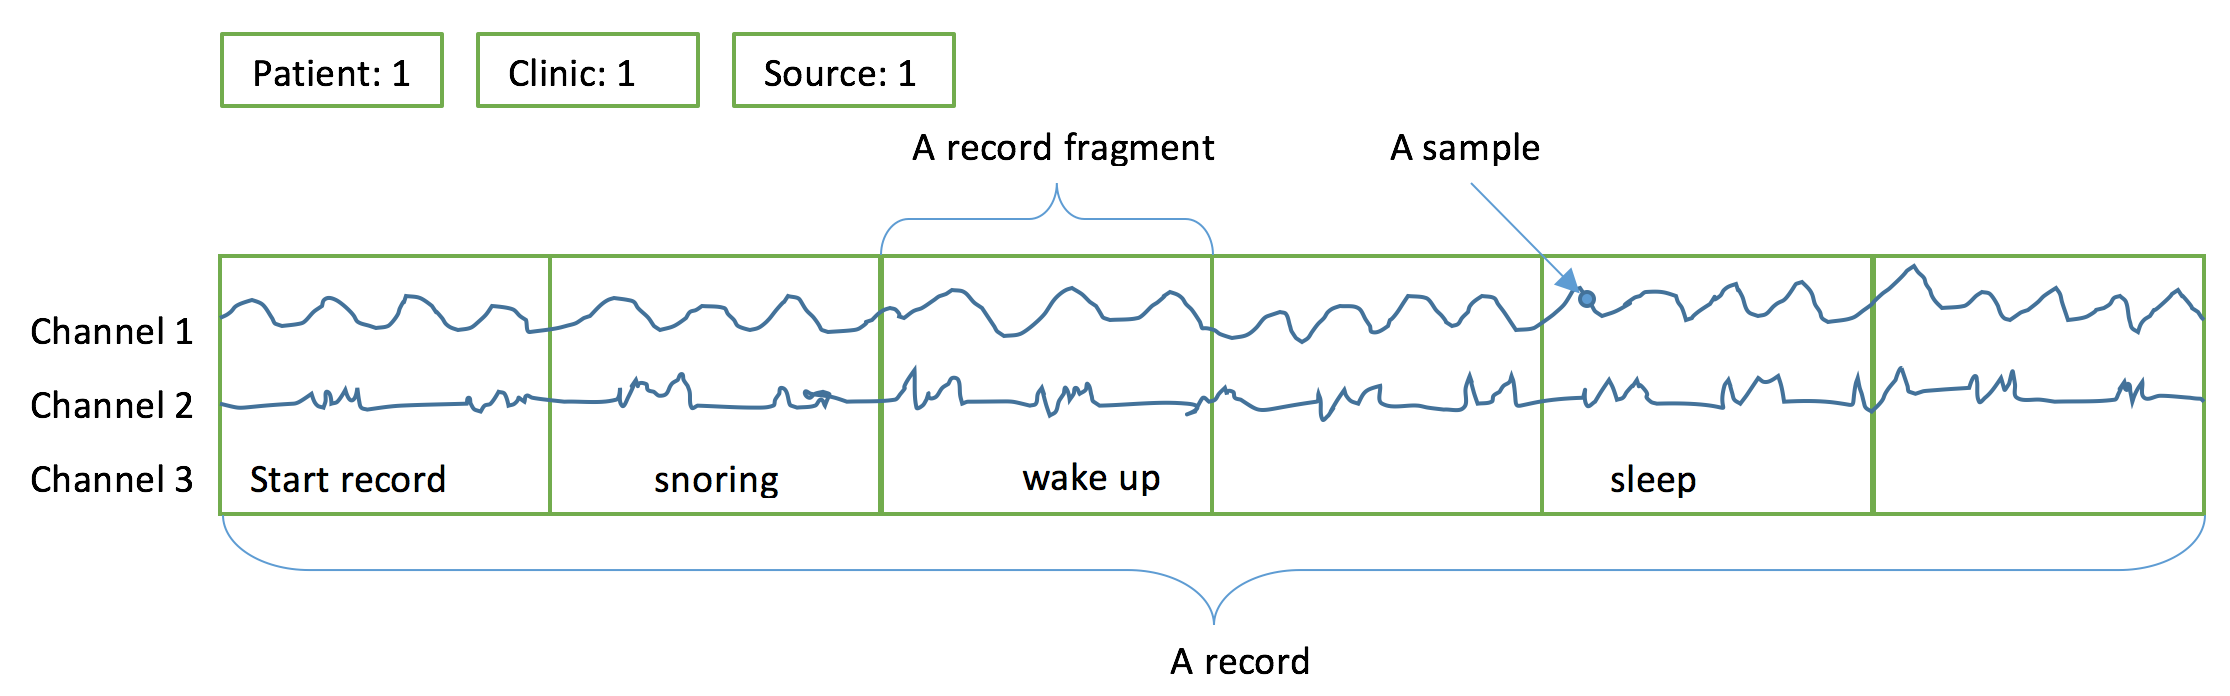
\includegraphics[width=1.0\textwidth]{Figures/ARecord.png}
    \caption{Example of a recording from a source}
    \label{fig:Figures/RecordingExample}
\end{figure}
One of the most important part of the conceptual data modeling is to define relationships between the classified entities. In this part, the Object Role Modeling (ORM) is used for presenting the relationships between entities. ORM is chosen because it is a method for designing and querying database models at the conceptual level, and easy to validate and evolve\cite{ORMdotNET}.\\
A short history of ORM, the term “object-role model” is given in Eckhard Falkenberg’s doctoral thesis which was published in 1976\cite{Wiki_ORM}. ORM is a very good method which is used for designing and querying database models at the conceptual level. ORM uses natural language, as well as diagrams to simplify the design process. With ORM, a conceptual approach to modeling is provided by expressing the model in terms of natural concepts, such as objects and roles. Elementary facts are fundamental for ORM. These elementary facts are expressed in diagrams, and are verbalized into natural language. Nevertheless, modeling, transforming, and querying data from a domain becomes much easier with the help of the “fact-based” approach. ORM is easily to understand by non-technical users, because it is attribute free. It is to say, all the facts are treated as relationships. Moreover, when drawing a graphic, it is more expressive and easier to be understood by people without technical background. Last but not least, avoiding attributes in the database model does not only improve the semantic stability, but also enables the verbalization into natural language.\\
Based on the classified entities, facts of the database system can be expressed as below:
\begin{adjustwidth}{1cm}{}
•	Source has Recording for Patient(Person) at Clinic.\\
•	Recording for Patient(Person) is produced by Physician/Patient(Person) by using Source.\\
•	Patient/Physician(Person) at Clinic uses Source to produce Recording.\\
•	Physician(Person) work for Clinic.\\
•	Patient(Person) belongs to Clinic.
\end{adjustwidth}
There is another view of the conceptual data model where the entity Recording is treated as a relationship. Facts that respected to this view are as below:
\begin{adjustwidth}{1cm}{}
•	Source is used by Patient(Person) at Clinic.\\
•	Patient(Person) at Clinic uses Source.\\
•	Physician(Person) uses Source for Patient(Person).\\
•	Physician(Person) work for Clinic.\\
•	Patient(Person) belongs to Clinic.
\end{adjustwidth}
The second view is easy to read. However, when transform this view into a logical model, a product from “uses” must be defined, and it is a Recording with respect to the first view. It is to say, there are a lot of possible views when doing conceptual data modeling. It is difficult to say which is the best view to use. Therefore, these views need to be integrated. Toby et.al[cite] also suggest four steps for conceptual schema integration, they are pre-integration analysis, comparison of schema, conformation of schema, merging and restructuring of schema. Integration for the views in this part is simple. The first view is extended from the second view, hence, it has a better presentation compared with the second view.\\
Figure \ref{fig:Figures/ConceptDB1} presents the first view where Recording is presented as an entity, while in Figure \ref{fig:Figures/ConceptDB2}, Recording is presented as a relationship. As argued in view integration, Figure \ref{fig:Figures/ConceptDB1} illustrates the conceptual model of the database system. Only notations that are used in the thesis, are described. The other notations which are irrelevant to this design, can be found in the ORM article written by Terry Halpin\cite{ORMdotNET2}.\\
Figure \ref{fig:Figures/USEDORM} presents the used notations, which are uniqueness constraint, object type shapes, shapes and readings for predicates and roles, sub-typing, and mandatory role constraint.\\
\begin{figure}[ht]
    \centering
    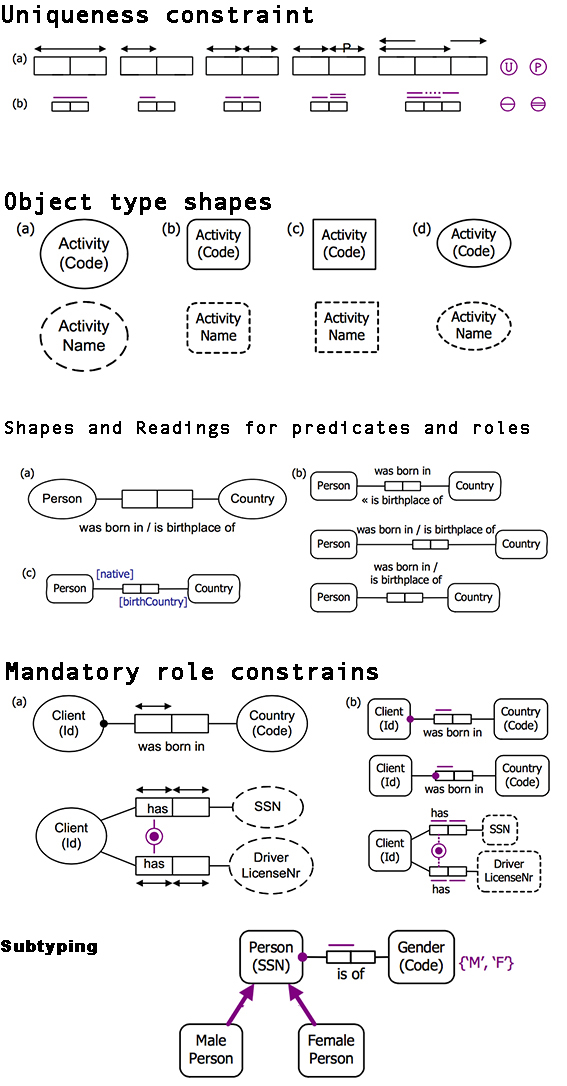
\includegraphics[width=0.7\textwidth]{Figures/USEDORM.png}
    \caption{View where Recording is presented as an entity}
    \label{fig:Figures/USEDORM}
\end{figure}
In the figure, \textbf{uniqueness constraint} (a) is used in the first version of ORM, while (b) is used in the second version(ORM2). These notations which are many to many (n:m), one to many (1:n), one to one (1:1), one to one which is primary, and a combination of these constraints respectively to the figure.\\
\textbf{Object type shapes} (a) is used in ORM, while (b), (c), and (d) is used in ORM2. As presented in ORM2 article\cite{ORMdotNET2}, after a survey of 18 experts, 12 of them prefer (b), 5 of them prefer (d), and the last one prefer (c). Hence, (c) is chosen as default type shape for objects, while (c) and (d) are the alternatives.\\
\textbf{Shapes and reading for predicates and roles} (a) are used in ORM, and (b), (c) is used in ORM2. There is a bi-directional read for predicates and roles.\\
Mandatory role constrains are indicated by a solid dot. (a) is notations for ORM, and (b) is for ORM2.\\
\textbf{Sub-typing notation} presents the hierarchy between objects.\\
\begin{figure}[ht]
    \centering
    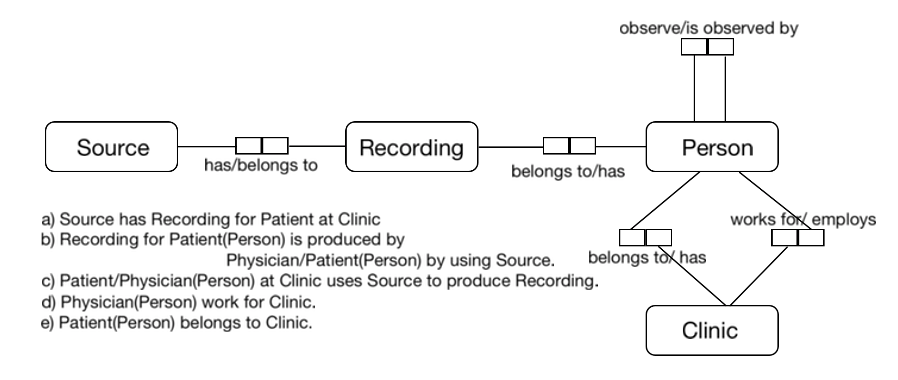
\includegraphics[width=1.0\textwidth]{Figures/ConceptDB1.png}
    \caption{View where Recording is presented as an entity}
    \label{fig:Figures/ConceptDB1}
\end{figure}
\begin{figure}[ht]
    \centering
    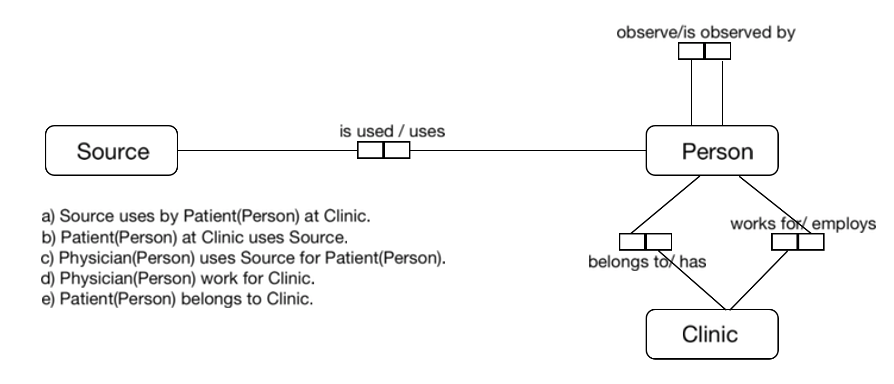
\includegraphics[width=1.0\textwidth]{Figures/ConceptDB2.png}
    \caption{View where Recording is presented as a relationship}
    \label{fig:Figures/ConceptDB2}
\end{figure}
\section{Logical data modeling}
The logical data model describes the abstract structure of the database system. Therefore, it is independent of a particular database management system. That means it does not describe what data types should be used, which technologies can be used such that queries can execute fast, etc., but it should describe tables (entities) and columns (attributes), relationships, etc., in which the primary keys for columns and the reference keys must be specified. The logical data model also the presents relationships between the entities. Therefore, all entity relationships need to be specified. Then, all attributes for each entity must be carefully identified. Since this thesis takes the future growth of data and meta-data of OSA database into considering, it is essential for finding all possible attributes for the specified entities that are described in Section 2. After that, a set of function dependences (FDs) can be derived from the relationships and attributes. Finally, database normalization need to be performed such that the database can be accurate, fast, and efficient. Subsection 3.1 presents the relationships between classified entities. In this subsection, many-to-many relationships are also resolved. Normalization and step by step to normalize are discussed and presented in Subsection 3.2.
\subsection{Relationships between different entities}
Based on the facts that are presented in Section 2, the data relationships are described as the following assertions:
\begin{adjustwidth}{1cm}{}
•	Each Source has many Recordings, but one Recording belongs to only one Source.\\
•	Each Source can be used by many different Person, and each Person can use many different Sources.\\
•	Each Source can be used by many different Clinics, and each Clinic can use many difference Sources.\\
•	Person has many Recordings, but one Recording belongs to only one Person.\\
•	Person collects many Recording, but one Recording is collected by only one Person.\\
•	Each Recording is produced by a Source, for a Person at a certain Clinic at a certain time.\\
•	Each Person works/belongs to many Clinics, and each Clinic employs/has many Person.\\
•	Each Person (Physician) observers many Persons (Patient), and many Person(Patient) are observed by a Person(Physician).
\end{adjustwidth}
These relationships can be divided into three groups: binary relationships, binary recursive relationships and ternary (or n-ary) relationships. Figure \ref{fig:Figures/RelationshipBinary} and \ref{fig:Figures/NaryAndRecursive} present these relationships by using ORM notations.\\
\begin{figure}[ht]
    \centering
    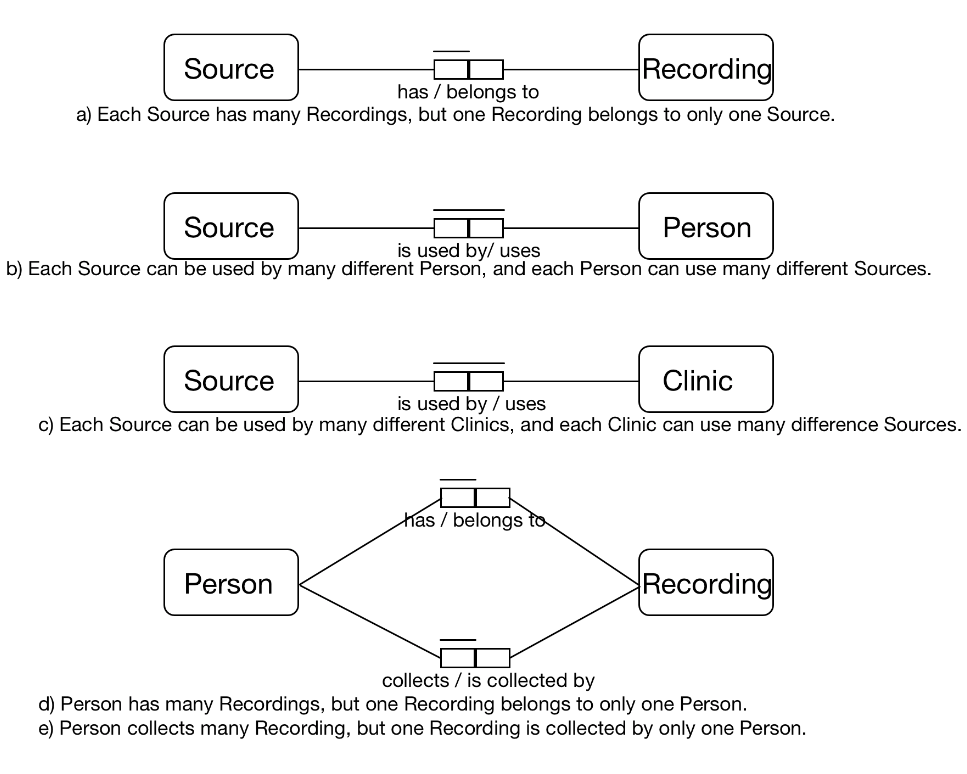
\includegraphics[width=1.0\textwidth]{Figures/RelationshipBinary.png}
    \caption{Binary relationships}
    \label{fig:Figures/RelationshipBinary}
\end{figure}
\begin{figure}[ht]
    \centering
    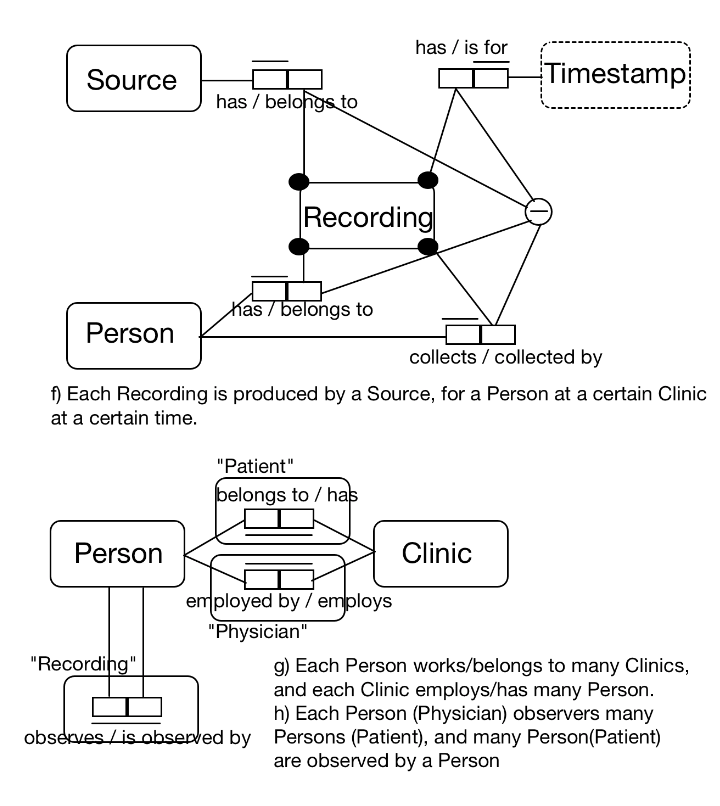
\includegraphics[width=1.0\textwidth]{Figures/NaryAndRecursive.png}
    \caption{Recursive and n-ary relationships}
    \label{fig:Figures/NaryAndRecursive}
\end{figure}
Foreign keys are easily derived from binary relationships. If there is a one-to-one binary relationship, the key of either entity can be used as a foreign key in the table of the other entity. If there is a one-to-many binary relationship, the foreign key must appear on the “many” side, since the “many” side presents the child entity. A many-to-many binary relationship must be resolved, since the relational database management system cannot hold this relationship. An easiest way to resolve a many-to-many binary relationship is to convert this relationship into a new entity, in which each old entity has a one-to-many binary relationship with the new entity. In this thesis, it is natural to see that most of the many-to-many binary relationships from the assertions can be resolved by using the Recording entity as a new entity between the old entities. Physician and Patient can be used as new entities for relationships “works/belongs to” and “employ/has” respectively in the assertion “Each Person works/belongs to many Clinics, and each Clinic employs/has many Person”. As a result, the new entities must contain foreign keys that refer to parent entities.\\
In a binary recursive relationship between two Persons (a Person observes a Person), a foreign key refers to a column which identifies the referred Person. The 4-ary relationship “Each Recording is produced by a Source, for a Person at a certain Clinic at a certain time” presents that Recording is depended on a Source, a Person and a Clinic at a specific time, therefore it must contain the primary keys of these entities as foreign keys.\\
A multivalued dependence $A \twoheadrightarrow B$ is defined whenever a relation has two tuples that agree in all the attributes of X, then their Y components can be swapped and get to new tuples that also in the relation. In entity Recording, a recording id $\twoheadrightarrow$ all of the annotations attributes. That is, there are possible to have multiple annotations at the same timestamp, and many timestamp could have the same notation text. Therefore, entity Recording has one multivalued dependence which is recording id $\twoheadrightarrow$ annotation onset, annotation duration, annotation timekeeping, annotation text.
Most of attributes for each entity can be taken from Table \ref{tab:entitiesAttributes}. In terms of future analysis, some of attribute are added to Person. Table \ref{tab:EntitiesFDs} presents the entities together with their attributes and FDs, and it is a result of the analysis. In this table, each attribute of a entity is given an alias for saving writing when finding primary keys and decomposition.
\begin{table}[ht]
\begin{center}
\begin{tabular}{ |p{1.5cm}||p{5cm}|p{6.5cm}|  }
 \hline
 Entities& Attributes& Function dependents\\
 \hline
 Source& source identifier (A), source name (B), channel number (C), channel name (D), metric (E), transducer type (F), physical maximum (G), physical minimum (H), digital maximum (I), digital minimum (J), EDF reserved compatible (K), source type (L)& \textbf{A,C} $\rightarrow$ D, E, F, G, H, I, J, K\newline \textbf{A} $\rightarrow$ B, L\\
 \hline
 Recording& recording id (A), source identifier (B), channel number (C), id person collects recording (D), id person own recording (E), recording timestamp (F), recording description (G), frequency (H), pre-filtering (I), sample timestamp (J), sample value (K), annotation onset (L), annotation duration (M), annotation timekeeping (N), annotation text (O), used equipment (P), EDF reserved (Q)& \textbf{A} $\rightarrow$ B, C, D, E, F, G, H, I, L, M, N, O, P, Q\newline \textbf{B,C,D,E,F} $\rightarrow$ A, G, H, I, L, M, N, O, P, Q\newline \textbf{A,J} $\rightarrow$ K\newline \textbf{A} $\twoheadrightarrow$ L,M,N,O\\
 \hline
 Person& person id (A), name (B), city (C), phone number (D), email (E), gender (F), data of birth (G), age (H), height(I), weight(J), BMI(K), clinic code patient(L), clinic code physician(M), other health issues (N), title in clinic(O)& \textbf{A} $\rightarrow$ B, C, D, E, F, G, H\newline \textbf{A,L} $\rightarrow$ I, J, K, N\newline \textbf{A,M} $\rightarrow$ O\\
 \hline
 Clinic& clinic code (A), name (B), address (C), phone number (D), email (E)& \textbf{A} $\rightarrow$ B, C, D, E\\
 \hline
\end{tabular}
\end{center}
\caption{OSA entities with their attributes and FDs}
\label{tab:EntitiesFDs}
\end{table}

Based on the defined function dependents of the entities, primary keys of these entities can be found by following these steps\cite{INF3100_Recipe_book}:
\begin{adjustwidth}{1cm}{}
With FDs belong to a relation/entity R:\\
1. Let X = a set of attributes that are not exist in any right hand side if the FDs.\\
2. Expand systematic X in every possible ways with the attributes that occur at least one on left hand side of FDs.\\
Compute closure X+ for each such X until X+ are all attributes.\\
If X+ are all attributes in R, check that whatever an attribute A is chosen in X, (X-A)+ is not a set of all attributes of R.\\
If that is the case, X is a candidate (primary) key.
\end{adjustwidth}
A algorithm, that is used for computing a closure of the attribute set with respect to FDs, is as follow\cite{INF3100_Recipe_book}:
\begin{adjustwidth}{1cm}{}
Let X is a set of attributes in relation, and X+ is a closure of X.\\
1. T := X\\
2. As long as T changed, if there is a FD A $\rightarrow$ B in FD set, where A is a subset of T, T:=T$\cup$B\\
3. X+ := T
\end{adjustwidth}

\textbf{Source}\\
A and C are not presented in the right hand side of the two FDs. After computing AC+, all of attributes are retrieved. There is no need to expand AC when it is a candidate key.
Therefore, AC is the only candidate key of this entity\footnote{To be easy to follow, entity, relation, and table are used alternatively.}.\\
\textbf{Recording}\\
J are not presented in the right hand side of the FDs. After computing J+, none of attribute are retrieved. Expand J with A, after computing AJ+, none of attribute are retrieved. Therefore, AJ is a candidate key of this entity. Repeat the expanding process, an other candidate key can be found, which is BCDEFJ. Therefore, this table has two candidate keys which are AJ and BCDEFJ.\\
\textbf{Person}\\
A, L, and M are not presented in the right hand side of the FDs. After computing ALM+, all of attribute are retrieved. Therefore, ALM is the only candidate key of this entity.\\
\textbf{Clinic}\\
All of other attributes depend on A, therefore A is the only candidate key of this entity.\\
Table \ref{tab:entitiesPrimaryKey} presents the results after performed the key-finding algorithms.\\

\begin{table}[ht]
\begin{center}
\begin{tabular}{ |p{3cm}||p{10cm}|}
 \hline
 Entity& Primary key / candidate key\\
 \hline
 Source& (source identifier, channel number) as AC\\
 \hline
 Recording& (recording id, sample timestamp) as AJ, and (source identifier, channel number, id person collects recording, id person own recording, recording timestamp) as BCDEFJ\\
 \hline
 Person& (person id, clinic code patient, clinic code physician) as ALM\\
 \hline
 Clinic& (clinic code) as A\\
 \hline
\end{tabular}
\end{center}
\caption{Classified entities with their primary/candidate keys}
\label{tab:entitiesPrimaryKey}
\end{table}
\subsection{Normalization}
Normalization is essential for relational database tables in terms of integrity, maintainability and performance. After classifying, identifying attributes and relationships for entities, which is a tuple in a table in relational database, the table may produce redundant data when the entities are stored in a database system, if the table is not normalized. Moreover, it may take long time to search some particular rows due to the redundant data. Update and delete are extremely expensive when the redundant data are large. These costs are caused by the fact that the database management system must do an update or a delete operation for each of the redundant data. A method to break a large redundant table into many compact, non-redundant tables to avoid the high costs of redundant data, is called normalization. After normalization, the database would become much more reliable and efficient. Table \ref{tab:FamousNF} present a short summary of famous normal forms which are derived from the INF3100(Database System course)\cite{INF3100} lecture.
\begin{table}[ht]
\begin{center}
\begin{tabular}{ |p{3cm}||p{5cm}|p{5cm}|  }
 \hline
 Normal form& Definition& Characteristic\\
 \hline
 First normal form (1NF)&- All columns contain only atomic values\newline
 - Each column can have only one value (or nil) for each row&- Repeating groups in a table are eliminated\newline
 - A primary key is used for identifying each set of related data\\
 \hline
 Second normal form (2NF)&is 1NF, with FD: X $\rightarrow$ A, where X is a set of attributes and A is an attribute. One of the following must be hold:\newline
 - X is a super key\newline
 - A is a key-attribute\newline
 - X is not a subset of any candidate keys&the same as 1NF, plus:\newline
 - All non-key attributes are fully FD on the primary key\\
 \hline
 Third normal form (3NF)&is 2NF, with FD: X $\rightarrow$ A, where X is a set of attributes and A is an attribute. One of the following must be hold:\newline
 - X is a super key\newline
 - A is a key-attribute&the same as 2NF, plus:\newline
 - There is no transitive FDs\\
 \hline
 Boyce-Codd normal form (BCNF)&is 3NF, with FD: X $\rightarrow$ A, where X is a set of attributes and A is an attribute. One of the following must be hold:\newline
 - X is a super key&the same as 3NF, plus:\newline
 - All FDs are super keys\\
 \hline
 Fourth normal form (4NF) &is BCNF, with MVD: X $\twoheadrightarrow$ Y, where X is a set of attributes and Y is an other set of attributes. One of the following must be hold:\newline
 - X is a super key&the same as BCNF, plus:\newline
 Y is a subset of X, or X and Y together form the whole set of attributes of the relation\\
 \hline
\end{tabular}
\end{center}
\caption{An overview of normal forms}
\label{tab:FamousNF}
\end{table}
Although 3NF eliminates most of the anomalies in databases, there are still some anomalies when a table has multiple overlapping candidate keys. The BCNF can eliminate these anomalies, but the BCNF can not solve the multivalued dependence problem. Therefore, 4NF is chosen as the highest form for the design. For each table (entity) in Table \ref{tab:EntitiesFDs}, a procedure to check and normalize these table is presented as follow\cite{INF3100_Recipe_book}:
\begin{adjustwidth}{1cm}{}
For each entity with its FDs and MVDs:\\
1. For each of MVDs X $\twoheadrightarrow$ Y, decompose R to R1(XY) and R2(XZ) where Z is all attributes in R and not in XY.\\
2. For each of FDs, BCNF checking and decomposing processes as follow\cite{INF3100_Recipe_book}:
For each entity with its FDs:\\
2.1. All candidate keys are listed.\\
2.2. All the right hand side with multiple attributes must be split into atomic FDs (only one attribute on the right hand side).\\
2.3. For each atomic FD X$\rightarrow$A, check the FD with the rules in Table \ref{tab:FamousNF} to find the normal form of this FD.\\
The normal form of the entity (relation) is the lowest normal form of the FDs.
\end{adjustwidth}
Once the normal form of the table is found, if it is not at the desirable normal form, decomposition can be taken place as follow\cite{INF3100_Recipe_book}:
\begin{adjustwidth}{1cm}{}
Assume there is a relation R with FDs F that breaks BCNF:\\
1. If $X \rightarrow A$ breaks BCNF, compute X+, then decompose R into S and T, where S:=X+, T:=X$\cup$(R-X+).
2. Repeat 1 with the new relations (in this case are S,T) until all relations are decomposed to BCNF.
\end{adjustwidth}
\textbf{Source}\\
There is no MVD in this table. Candidate key of the table is AC.\\
This table has two FDs, which are \textbf{AC} $\rightarrow$ DEFGHIJK and \textbf{A} $\rightarrow$ BL.\\
After split, the table has $F=\{AC \rightarrow D, AC \rightarrow E, AC \rightarrow F, AC \rightarrow G, AC \rightarrow H, AC \rightarrow I, AC \rightarrow J, AC \rightarrow K, A \rightarrow B, A \rightarrow L\}$.
- $A \rightarrow B$: The left hand side of this FD is not a super key, therefore, it breaks BCNF, This FD is neither 3NF, because the right hand side of FD is not an attribute in candidate key. The FD is not 2NF, since the right hand side is a subset of candidate key. Hence, the FD is 1NF.\\
Since 1NF is the lowest normal form, there is no need to scan the other FDs to find the normal form of the table. The normal form of a table is the lowest normal form of its FDs. Therefore, the normal form of table Source is 1NF.\\
Let a new relation R1 = A+ = (ABL); an other relation R2 = A$\cup$(R-R1) = (ACDEFGHIJK). After the composition, A is a primary key of table R1(ABL) as SensorSource(source identifier, source name, source type), and AC is a primary key of table R2(ACDEFGHIJK) as Channel(source identifier, channel number, channel name, metric, transducer type, physical maximum, physical minimum, digital maximum, digital minimum, EDF reserved compatible). Therefore, this composition is in BCNF.\\
\textbf{Recording}\\
This table has one MVD which is A $\twoheadrightarrow$ LMNO. This MVD can be split into two tables R1 and R2. R1 contains all attributes from the MVD, that is ALMNO; R2 contains the attributes from the left hand side of the MVD and the attributes that do not exists on the right hand side of the MVD, they are ABCDEFGHIJKPQ. R2 is named Recording; R1 is named Annotation. To decompose the table to 4NF, the Recording need to be decomposed to BCNF with respect to the FDs.\\
Table Recording has two candidate keys which are AJ and BCDEFJ. The table has three FDs, which are \textbf{A} $\rightarrow$ BCDEFGHILMNOPQ, \textbf{BCDEF} $\rightarrow$ AGHILMNOPQ, and \textbf{AJ} $\rightarrow$ K.\\
After split, the table has $F=\{A \rightarrow B, A \rightarrow C, A \rightarrow D, A \rightarrow E, A \rightarrow F, A \rightarrow G, A \rightarrow H, A \rightarrow I, A \rightarrow L, A \rightarrow M, A \rightarrow N, A \rightarrow O, A \rightarrow P, A \rightarrow Q, BCDEF \rightarrow A, BCDEF \rightarrow G, BCDEF \rightarrow H, BCDEF \rightarrow I, BCDEF \rightarrow L, BCDEF \rightarrow M, BCDEF \rightarrow N, BCDEF \rightarrow O, BCDEF \rightarrow P, BCDEF \rightarrow Q, AJ \rightarrow K\}$.
- $A \rightarrow B$: The left hand side of this FD is not a super key, therefore, it breaks BCNF. This FD is neither 3NF, because the right hand side of FD is not an attribute in candidate key. The FD is not 2NF, since the right hand side is a subset of candidate key. Hence, the FD is 1NF.\\
Since 1NF is the lowest normal form, there is no need to scan the other FDs to find the normal form of the table. Therefore, the normal form of table Source is 1NF.\\
Let a new relation R1 = A+ = (ABCDEFGHIPQ); an other relation R2 = A$\cup$(R-R1) = (AJK). After the composition, A and BCDEF are primary keys of table R1, AJ is primary key of R2, and A is primary key of Annotation(ALMNO). Since A depends on BCDEF, and LMNO depends on A, the composition is satisfy the 4NF.\\
The Recording table is split into R1(ALMNO) as Annotation(recording id, annotation onset, annotation duration, annotation timekeeping, annotation text), R2(ABCDEFGHIPQ) as Record(recording id, source identifier, channel number, id person collects recording, id person own recording, recording timestamp, recording description, frequency, pre-filtering, used equipment, EDF reserved), and R3(AJK) as Sample(recording id, sample timestamp, sample value).\\
However, in Annotation table, a many-to-many relationship between records and annotations need to be solved. The many-to-many relationship exists, because there is a transitive relationship between records for a source an its annotations. That is, one source has one set of annotations for all channels belong to the source at a specific timestamp. Furthermore, a record is defined by a source id, channel is, patient id, physician id, and timestamp. Therefore, one record has many annotations, and one annotations belong to many records. To solve the many-to-many relationship, Annotation table need to be split into RecordAnnotation(record id, annotation id) and Annotation(annotation id, onset, duration, timekeeping, annotation text).\\
\textbf{Person}\\
There is no MVD in this table. Candidate key of the table is ALM.\\
This table has three FDs, which are \textbf{A} $\rightarrow$ BCDEFGH, \textbf{AL} $\rightarrow$ IJKN, and \textbf{AM} $\rightarrow$ O.\\
After split, the table has $F=\{A \rightarrow B, A \rightarrow C, A \rightarrow D, A \rightarrow E, A \rightarrow F, A \rightarrow G, A \rightarrow H, AL \rightarrow I, AL \rightarrow J, AL \rightarrow K, AL \rightarrow N, AM \rightarrow O\}$.
- $A \rightarrow B$: The left hand side of this FD is not a super key, therefore, it breaks BCNF, This FD is neither 3NF, because the right hand side of FD is not an attribute in candidate key. The FD is not 2NF, since the right hand side is a subset of candidate key. Hence, the FD is 1NF.\\
Since 1NF is the lowest normal form, there is no need to scan the other FDs to find the normal form of the table. Therefore, the normal form of table Source is 1NF.\\
Let a new relation R1 = A+ = (ABCDEFGH); an other relation R2 = A$\cup$(R-R1) = (AIJKNLMO). After the composition, A is a primary key of table R1, but AL and AM are not primary keys of table R2. Therefore, the composition need to be repeated on R2. Let a new relation R3 = AL+ = (ALIJKN); an other relation R4 = AL$\cup$(R2-R3) = (ALMO). After the composition, AL is a primary key of table R3, and AM is a primary key of table R4. However, R4 and R3 is sub-object of R1, hence, R4 does not need to take L. Therefore, the decomposition is in BCNF with relations R1(ABCDEFGH) as Person(person id, name, city, phone number, email, gender, data of birth, age), R3(ALIJKN) as Patient(person id, clinic code patient, height, weight, BMI, other health issues), and R4(AMO) as Physician(person id, clinic code physician, title in clinic).\\
\textbf{Clinic}\\
Clinic has only one FD which is also the primary key of the relation. Therefore, it is automatic in BCNF.\\
\begin{figure}[ht]
    \centering
    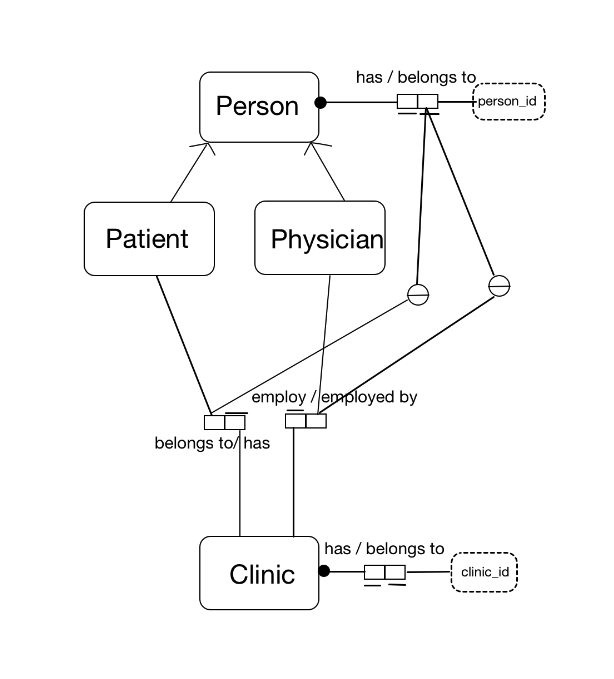
\includegraphics[width=1.0\textwidth]{Figures/LogicalModelDB1.png}
    \caption{Logical model of the OSA database - Person and Clinic}
    \label{fig:Figures/LogicalModelDB1}
\end{figure}
\begin{figure}[ht]
    \centering
    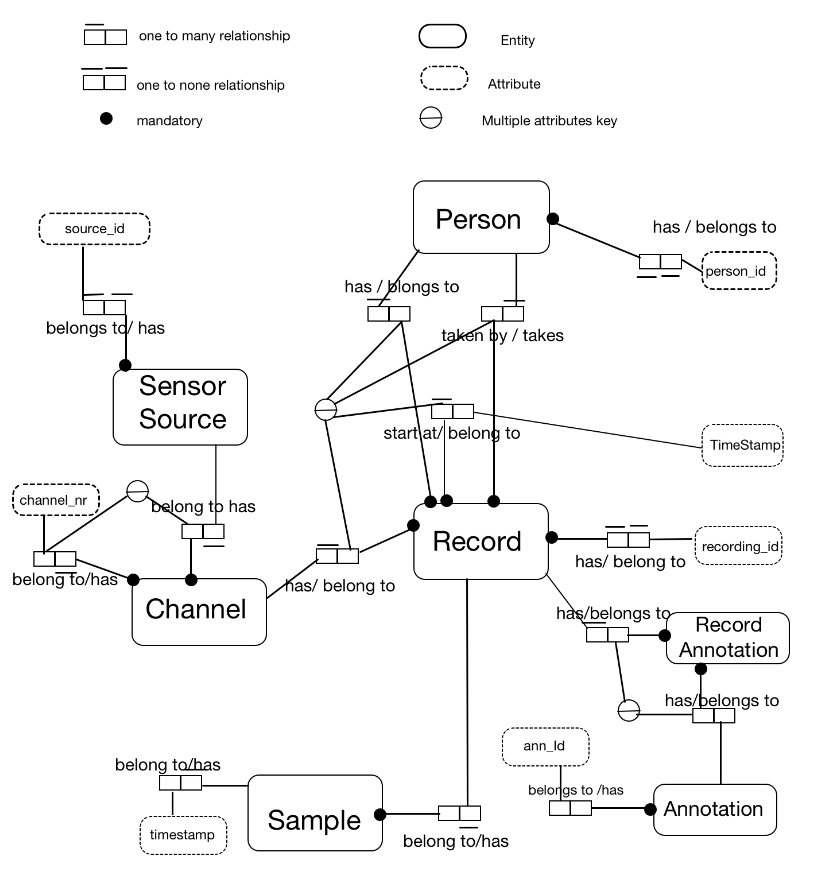
\includegraphics[width=1.0\textwidth]{Figures/LogicalModelDB2.png}
    \caption{Logical model of the OSA database - Source and Recording}
    \label{fig:Figures/LogicalModelDB2}
\end{figure}
Figure \ref{fig:Figures/LogicalModelDB1} and \ref{fig:Figures/LogicalModelDB2} presents a summary of the logical model of the database design after decomposition. In this figure, non-key attributes are hidden to maximize the abstraction.
\section{Physical data modeling}
The logical data model, which is presented in Figure \ref{fig:Figures/LogicalModelDB1} and \ref{fig:Figures/LogicalModelDB2}, is a platform independent model. This model can be implement on a workstation computer or even mobile platform as long as these platforms have a database management system. Since this thesis chooses the Android operation system as a platform to implement the design, the SQLite database manage system is chosen for modeling the physical data. An overview of SQLite database management system is discussed in Subsection 4.4.1. Subsection 4.4.2 presents the transformation of logical data model to physical data model.
\subsection{SQLite database management system}
As presented in SQLite site\cite{SQLITEORG}, SQLite is an embedded SQL database engine. It does not support client-server process as other database management systems do. However, other SQL database elements that are needed for this design are fully supported. They are multiple tables, indices, triggers, and views. In SQLite, all the mentioned elements are included in a single file on disk. In terms of opening file for doing analysis and modifying, using a database management is much better than using buffer and file functions offered by a programming language.\\
SQLite has five data storage classes that can be used for the physical data modeling.
\begin{adjustwidth}{1cm}{}
•	NULL: The value is a NULL value.\\
•	INTEGER: The value of this type is a signed integer. Depend on the magnitude of the stored value, it could be one, two, three, four, six, or eight bytes in size.\\
•	REAL: The value of this type is a floating point value following the IEEE floating point number. This type is eight bytes in size.\\
•	TEXT: Unlike the other database management systems, SQLite has only one type for storing a text string. The text could be encoded as UTF-8, UTF-16 big-endian, or UTF-16 little endian.\\
•	BLOB: The value of the type is BLOB(Binary Large OBject) stored in exactly the same format as it is provided to the database.
\end{adjustwidth}
In SQLite, the term of “datatype” is not used, but “storage class”, since data are dynamically stored in the system. Therefore, the data need to be converted before storing, or using. However, at an abstract level, the two terms present data type. Hence, these terms can be used interchangeably.
\subsection{Transforming the logical data model to SQL}
As presented in Figure \ref{fig:Figures/LogicalModelDB1} and \ref{fig:Figures/LogicalModelDB2}, there are nine entities that must be transformed into tables. The names of these entities are also used for the corresponding tables in SQLite. Attributes of the entities become columns in the tables, and the relationships now become the foreign keys.
Tables \ref{tab:PersonTypeSQL} to \ref{tab:ChannelTypeSQL} present the attributes for each table with the explanation for each chosen type.
\begin{table}
\begin{center}
\begin{tabular}{ |p{4cm}|p{1.8cm}|p{6.2cm}|  }
 \hline
 \multicolumn{3}{|c|}{Person} \\
 \hline
 Columns& Data type & Explanation \\
 \hline
 person\_id& TEXT& person id can contains alphabetic character, not null\\
 name& TEXT& name is a string, can be null for anonymous\\
 city& TEXT& city is a string, can be null for anonymous\\
 phone\_nr& TEXT& phone number can contains +, can be null if not have\\
 email& TEXT& email is a string, can be null if not have\\
 gender& TEXT& gender can be a character or sometime a string, must be not null for later analysis\\
 date\_of\_birth& TEXT& date of birth is a string, must be not null for later analysis\\
 age& INT& age is an integer, can be null\\
 \hline
\end{tabular}
\end{center}
\caption{Transforming Person into SQLite table}
\label{tab:PersonTypeSQL}
\end{table}
\begin{table}
\begin{center}
\begin{tabular}{ |p{4cm}|p{1.8cm}|p{6.2cm}|  }
 \hline
 \multicolumn{3}{|c|}{Patient} \\
 \hline
 Columns& Data type & Explanation \\
 \hline
 person\_id& TEXT& foreign key to Person, not null\\
 clinic\_code& TEXT& foreign key to Clinic, not null\\
 patient\_code\_p& TEXT& Patient code in clinic, not null\\
 height& REAL& it must be floating number, can be null\\
 weight& REAL& it must be floating number, can be null\\
 BMI& REAL& it must be floating number, can be null\\
 other\_health\_issues& TEXT& it is a string, can be null\\
 \hline
\end{tabular}
\end{center}
\caption{Transforming Patient into SQLite table}
\label{tab:PatientTypeSQL}
\end{table}
\begin{table}
\begin{center}
\begin{tabular}{ |p{4cm}|p{1.8cm}|p{6.2cm}|  }
 \hline
 \multicolumn{3}{|c|}{Physician} \\
 \hline
 Columns& Data type & Explanation \\
 \hline
 person\_id& TEXT& foreign key to Person, not null\\
 clinic\_code\_f& TEXT& foreign key to Clinic, not null\\
 employee\_id& TEXT& Physician code in Clinic, not null\\
 title\_in\_clinic& TEXT& it is a string, can be null\\
 \hline
\end{tabular}
\end{center}
\caption{Transforming Physician into SQLite table}
\label{tab:PhysicianTypeSQL}
\end{table}
\begin{table}
\begin{center}
\begin{tabular}{ |p{4cm}|p{1.8cm}|p{6.2cm}|  }
 \hline
 \multicolumn{3}{|c|}{Clinic} \\
 \hline
 Columns& Data type & Explanation \\
 \hline
 clinic\_code& TEXT& it can contains text, not null\\
 name& TEXT& it is a string, can be null\\
 address& TEXT& it is a string, can be null\\
 phone\_nr& TEXT& phone number can contains +, can be null if not have\\
 email& TEXT& it is a string, can be null\\
 \hline
\end{tabular}
\end{center}
\caption{Transforming Clinic into SQLite table}
\label{tab:ClinicTypeSQL}
\end{table}
\begin{table}
\begin{center}
\begin{tabular}{ |p{4cm}|p{1.8cm}|p{6.2cm}|  }
 \hline
 \multicolumn{3}{|c|}{SensorSource} \\
 \hline
 Columns& Data type & Explanation \\
 \hline
 source\_id& TEXT& it can contains text, not null\\
 source\_name& TEXT& it is a string, can be null\\
 source\_type& TEXT& it is a string, can be null\\
 \hline
\end{tabular}
\end{center}
\caption{Transforming SensorSource into SQLite table}
\label{tab:SensorSourceTypeSQL}
\end{table}
\begin{table}
\begin{center}
\begin{tabular}{ |p{4cm}|p{1.8cm}|p{6.2cm}|  }
 \hline
 \multicolumn{3}{|c|}{Record} \\
 \hline
 Columns& Data type & Explanation \\
 \hline
 recording\_id& INT& unique long int from the system when created\\
 source\_id& TEXT& foreign key to SensorSource, not null\\
 channel\_nr& TEXT& together with SensorSource, it is foreign key to Channel, not null\\
 person\_collect& TEXT& foreign key to Person, not null\\
 person\_owner& TEXT& foreign key to Person, not null\\
 timestamp& INT& Unix time when the recording is started, not null\\
 description& TEXT& can be the applied position on the body, can be null\\
 frequency& REAL& collected at frequency, can be null\\
 used\_equipment& TEXT& other used equipment name, can be null\\
 EDF\_reverved& BLOB& reserved for EDF, byte array which may contains EDF+C, EDF+D, etc., can be null\\
 \hline
\end{tabular}
\end{center}
\caption{Transforming Record into SQLite table}
\label{tab:RecordTypeSQL}
\end{table}
\begin{table}
\begin{center}
\begin{tabular}{ |p{4cm}|p{1.8cm}|p{6.2cm}|  }
 \hline
 \multicolumn{3}{|c|}{RecordAnnotation} \\
 \hline
 Columns& Data type & Explanation \\
 \hline
 recording\_id& INT& foreign key to Record, not null\\
 annotation\_id& INT& foreign key to Annotation, not null\\
 \hline
\end{tabular}
\end{center}
\caption{Transforming RecordAnnotation into SQLite table}
\label{tab:RecordAnnotationTypeSQL}
\end{table}
\begin{table}
\begin{center}
\begin{tabular}{ |p{4cm}|p{1.8cm}|p{6.2cm}|  }
 \hline
 \multicolumn{3}{|c|}{Annotation} \\
 \hline
 Columns& Data type & Explanation \\
 \hline
 annotation\_id& INT& unique long int from the system when created, not null\\
 annotation\_onset& INT& when the annotation started, not null\\
 annotation\_duration& INT& how long an annotation last\\
 annotation\_timeKeeping& INT& if it is the first annotation in annotation lists\\
 annotation\_text& TEXT& text of the annotation\\
 \hline
\end{tabular}
\end{center}
\caption{Transforming Annotation into SQLite table}
\label{tab:AnnotationTypeSQL}
\end{table}
\begin{table}
\begin{center}
\begin{tabular}{ |p{4cm}|p{1.8cm}|p{6.2cm}|  }
 \hline
 \multicolumn{3}{|c|}{Sample} \\
 \hline
 Columns& Data type & Explanation \\
 \hline
 recording\_id& INT& foreign key to Record, not null\\
 sample\_timestamp& INT& Unix time, when it is created, not null\\
 sample\_value& REAL& it is a float number, not null\\
 \hline
\end{tabular}
\end{center}
\caption{Transforming Sample into SQLite table}
\label{tab:SampleTypeSQL}
\end{table}
\begin{table}
\begin{center}
\begin{tabular}{ |p{4cm}|p{1.8cm}|p{6.2cm}|  }
 \hline
 \multicolumn{3}{|c|}{Channel} \\
 \hline
 Columns& Data type & Explanation \\
 \hline
 source\_id& TEXT& foreign key to SensorSource, not null\\
 channel\_nr& INT& numerical order, not null\\
 channel\_name& TEXT& name of channel, not null\\
 metric& TEXT& metric, not null\\
 transducer\_type& TEXT& it is string, can be null\\
 physical\_maximum& REAL& physical maximum, can be null\\
 physical\_minimum& REAL& physical minimum, can be null\\
 digital\_maximum& INT& digital max, can be null\\
 digital\_minimum& INT& digital min, can be null\\
 pre\_filtering& TEXT& applied filtering on this channel, can be null\\
 EDF\_channel\_reserved& BLOB& EDF reserved\\
 \hline
\end{tabular}
\end{center}
\caption{Transforming Channel into SQLite table}
\label{tab:ChannelTypeSQL}
\end{table}
SQLite code for creating the Channel table is presented in Listing \ref{listing:SQLChannel}, creating code for the other tables can be found in Appendix XX.
\begin{code}[ht]
\begin{lstlisting}
    CREATE TABLE CHANNEL(
	   SOURCE_ID               TEXT NOT NULL,
	   CHANNEL_NR              INT NOT NULL,
	   CHANNEL_NAME            TEXT NOT NULL,
	   TRANSDUCER_TYPE         TEXT,
	   METRIC                  TEXT,
	   PHYSICAL_MAX            REAL,
	   PHYSICAL_MIN            REAL,
	   DIGITAL_MAX             INT,
	   DIGITAL_MIN             INT,
	   PREFILTERING            TEXT,
	   EDF_CHANNEL_RESERVED    BLOB,
	   PRIMARY KEY (CHANNEL_NR ,SOURCE_ID),
       FOREIGN KEY(SOURCEID) REFERENCES TABLE_SENSOR_SOURCE(SOURCE_ID)
	);
\end{lstlisting}
\caption[SQLite code for creating table Channel]{SQLite code for creating table Channel}
\label{listing:SQLChannel}
\end{code}\\
Figure \ref{fig:Figures/FinalTable} presents the final physical database model of the database system.
\begin{figure}[ht]
    \centering
    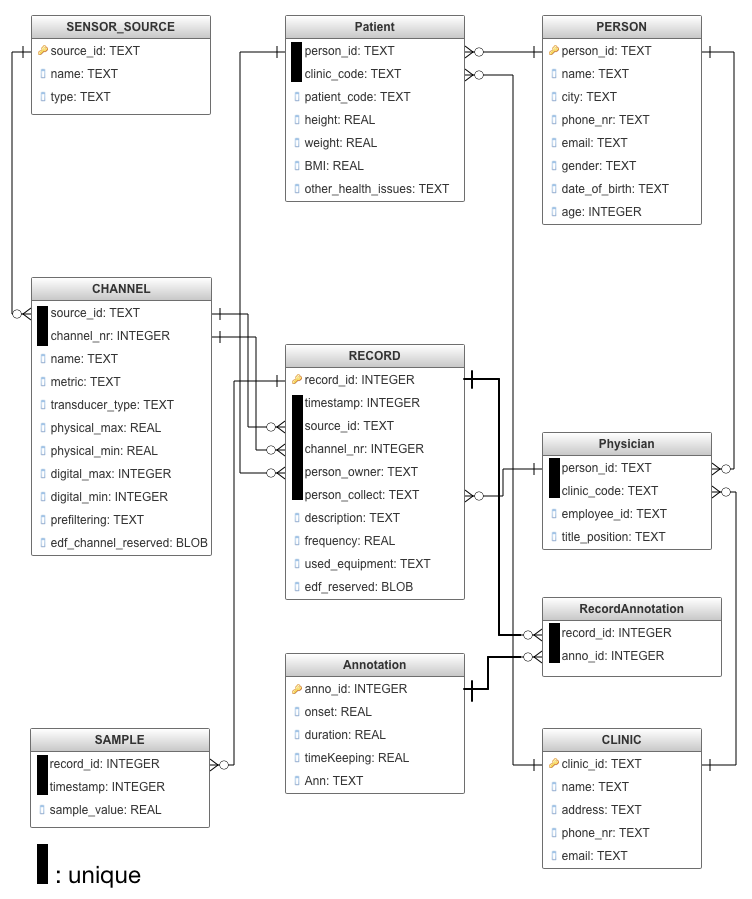
\includegraphics[width=1.0\textwidth]{Figures/FinalTable.png}
    \caption{Physical database model}
    \label{fig:Figures/FinalTable}
\end{figure}






